\chapter{Lecture 5}

%--- 信息 ----
\begin{center}
    讲师:王立威 \qquad
    课程时间:25.Mar.18th \qquad 
    笔记:25.June.7th
\end{center}

\bigskip

首先讨论了Pinsker不等式的证明方法,我直接放在了上一章当中. 

接下来看新的内容.  我们先来看一个例子来深入理解最短编码和信息熵之间的差距. 也就是要求整数和不要求整数之间的差距.  
\begin{example}
随机变量$X$,分布列$P=(0.01, 0.99)$ 
\begin{itemize}
    \item 信息熵$H(X) \approx 0.07 $\text{bit}.
    \item 最短编码1 bit.
\end{itemize}
\end{example}

事实上,我们有如下推论 
\begin{corollary}
    对于任意随机变量$X$,最短编码和信息熵的差严格小于1.
\end{corollary}

因此,通过差值来衡量编码效率是不合适的,我们应该使用比值来衡量.  另一方面,我们设定要传输可列次信息,也就是说存在一个i.i.d的序列$X_1, X_2,\dots$和$X$同分布.  我们传输这些信息时,不妨每$T$个打包成一组进行传输,可见这样一次传输的平均最小码长$l_{\min}$满足 
\[
l_{\min}(X_1, \dots, X_T) \le H(X_1, \dots, H_T) + 1 = T\cdot H(X) + 1
\] 

于是比值 
\[
\text{Ratio} = \dfrac{l_{\min}(X_1, \dots, X_T)}{H(X_1, \dots, H_T)} \le 1 + \dfrac{1}{T \cdot H(X)} = 1 + O\left(\dfrac{1}{T} \right)
\]

平均到编码每一个信息所需的长度有上界$\frac{T H(X) + 1}{T} \ra H(X)$.  因此,在$T \ra \infty$时,最终的平均码长应该趋于$H(X)$,而非$l_{\min}(X)$.  这也是为什么我们认为信息熵是一个本质的定义.  

值得指出,这样的操作在实际实践中会带来更大的时延. 

上面的模型其实对实际情况做了一个简化,也就是假设每个时刻的信息都是i.i.d的. 为了泛化我们的模型,我们应该将信源建模成随机过程(stochastic process)$\mathcal{X} = (X_t)_{t\ge 1}$,下面讨论这个模型.  

首先需要定义这个信源的平均码长. 
\begin{definition}[熵率]
    对于随机信源$\mathcal{X} = (X_t)_{t\ge 1}$,定义其\textbf{熵率}(entropy rate)为 
    \[
    H(\mathcal{X}):= \lim_{T \ra \infty} \dfrac 1T \cdot H(X_1, X_2, \dots, H_T)
    \]

    我们假定上述极限存在(这个技术细节过于琐碎,略去)
\end{definition}

另一种角度而言,我们也可以认为$H(\mathcal{X})$是每个时刻增加的新的信息. 
\begin{theorem}
    给定信源$\mathcal{X}= (X_t)_{t\ge 1}$,假设以下极限存在,那么下式成立. 
    \[
    H(\mathcal{X}) = \lim_{T \ra \infty} H(X_T | X_1, X_2, \dots, H_{T-1})
    \]
\end{theorem}
\begin{proof}
    注意到
    \[
    H(X_1, X_2, \dots, H_T) = H(X_1) + \sum_{i=2}^T H(X_i | X_{1 \sim (i-1)})
    \]

    使用数学分析(I)中的结论便可完成证明. 
\end{proof} 

接下来考虑连续随机变量的编码,但显然它没有所谓“最短平均码长”这一概念,我们只能先形式上给出一个熵的定义:
\begin{definition}[微分熵]
    对于连续型随机变量$X$,设其p.d.f.为$f(x)$,则定义其\textbf{微分熵}(differential entropy)为 
    \[
        h(X) := -\int_{\R} f(x) \log_2 f(x) \dx
    \]
\end{definition}

这个形式上定义并非单纯的望文生义,而是真正的有本之木!我们考虑连续型随机变量$X$对应的离散化版本$X_\Delta$,其中$\Delta > 0$是一个离散化的粒度. 具体而言,$X_\Delta$只取值于$k\Delta, \ (k \in \Z)$,并且 
\[
\Pr[X_\Delta = k\Delta] = \Pr[k \Delta \le X < (k+1)\Delta] = \int_{k \Delta }^{(k+1) \Delta} f(x) \dx
\]

可以得到如下的近似 
\begin{proposition}
    对于连续型随机变量$X$对应的离散化版本$X_\Delta$,有 
    \[
    h(X) + \log \dfrac{1}{\Delta} \approx H(X_\Delta)
    \]
\end{proposition}

另外,微分熵和香农熵在性质上也有一些不同的地方. 我们知道对于离散随机变量$X$,
\begin{itemize}
    \item 若$Y = X + c$,则$H(X) = H(Y)$
    \item 若$Z = aX (a>0)$,则$H(X) = H(Z)$
\end{itemize}

但对于连续随机变量和微分熵,对应的结论会变为
\begin{proposition}
    对于连续型随机变量$X$,若$Y = X + c$(其中$c$是常数),那么
    \[
    h(Y) = h(X)
    \]
\end{proposition}
\begin{proposition}
    对于连续型随机变量$X$,若$Z = aX$(其中$a>0$是常数),那么
    \[
    h(Z) = h(X) + \log a
    \]
\end{proposition}

下面举隅一例来计算其微分熵.
\begin{example}
    已知随机变量$X \sim \mathcal{N}(\mu, \sigma^2)$,求$h(X)$.
\end{example}
\begin{solution}
    我们记$X$的概率密度函数为$f(x)$,有 
\[
f(x) = \dfrac{1}{\sigma \sqrt{2\pi}} \exp\left\{
    -\dfrac{(x - \mu)^2}{2 \sigma^2}
    \right\}
\]
 
因此, 
\begin{align*}
    h(X) & = -\int_{-\infty}^{\infty} f(x) \log_2 f(x) \dx \\
    & = -\int_{-\infty}^{\infty} f(x) \cdot \left(
        -\log_2(\sigma \sqrt{2\pi}) - \dfrac{(x - \mu)^2}{2 \ln 2\cdot \sigma^2}
    \right) \dx \\
    & = \log_2(\sigma \sqrt{2\pi}) \int_{-\infty}^{\infty} f(x)\dx + \dfrac{1}{2 \ln 2\cdot \sigma^2} \int_{-\infty}^{\infty} (x-\mu)^2 f(x)\dx \\
    & = \log_2(\sigma \sqrt{2\pi}) + \dfrac{1}{2 \ln 2\cdot \sigma^2} \var(X) \\
    & = \log_2(\sigma \sqrt{2\pi}) + \dfrac{1}{2 \ln 2} \\ 
    & = \dfrac{1 + \log_2(\pi e \sigma^2)}{2}
\end{align*}

至此便得到了答案.
\end{solution}

% \begin{figure}[H]
%     \centering
%     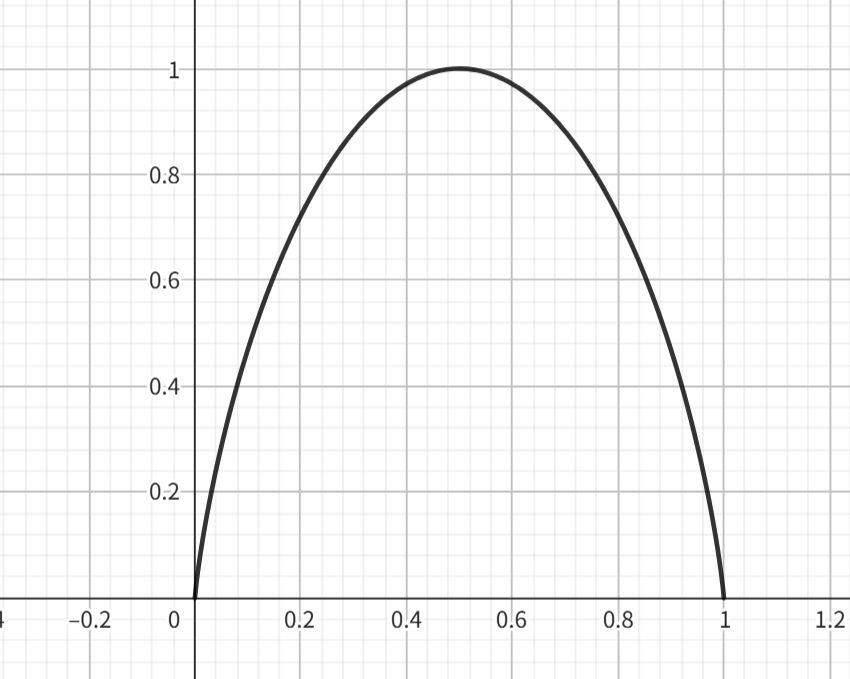
\includegraphics[width=.6\textwidth]{images/c2_1.png}
%     \caption{$H=x\log 1/x + (1-x)\log 1/(1-x)$的图像}
% \end{figure}